\documentclass[10pt]{amsart}
\usepackage[margin=1.4in]{geometry}
\usepackage[usenames,dvipsnames,cmyk]{xcolor} %load first
\usepackage{cancel}
\usepackage{amssymb,amsmath,enumitem,url}
\usepackage{graphicx,subfig}
\graphicspath{ {./images/} }

\newcommand{\D}{\mathrm{d}}
\newcommand{\I}{\mathrm{i}}
\DeclareMathOperator{\E}{e}
\DeclareMathOperator{\OO}{O}
\DeclareMathOperator{\oo}{o}
\DeclareMathOperator{\erfc}{erfc}
\DeclareMathOperator{\real}{Re}
\DeclareMathOperator{\imag}{Im}
\usepackage{tikz}
\usepackage[framemethod=tikz]{mdframed}
\theoremstyle{nonumberplain}

\mdtheorem[innertopmargin=-5pt]{sol}{Solution}
%\newmdtheoremenv[innertopmargin=-5pt]{sol}{Solution}
\definecolor{MichiganBlue}{HTML}{00274C}
\definecolor{MichiganYellow}{HTML}{FFCB05}  
\definecolor{NicePurple}{RGB}{75,56,76} %PrincePurple
\definecolor{NiceRed}{RGB}{230,37,52}
\definecolor{MidnightBlue}{rgb}{0.1, 0.1, 0.44}
\usepackage[colorlinks=true, linkcolor=MidnightBlue, citecolor=MidnightBlue, urlcolor=MidnightBlue]{hyperref}

\begin{document}
\pagestyle{empty}

\newcommand{\mline}{\vspace{.2in}\hrule\vspace{.2in}}

\noindent
\text{Hunter Lybbert} \\
\text{Student ID: 2426454} \\
\text{10-07-24} \\
\text{AMATH 567} \\

\title{\bf { Homework 2 } }


\maketitle
\noindent
Collaborators*: Nate Ward, Laura Thomas and Hailey Sparks \\
\\
\tiny
\text{*Listed in no particular order. And anyone I discussed at least part of one problem with is considered a colaborator.}
\normalsize
\mline
\begin{enumerate}[label={\bf {\arabic*}:}]
\item From A\&F: 1.2.12. \\
Show that a circle in the $z$ plane corresponds to a circle on the sphere.
(Note the remark following the reference to Figure 1.2.7 in Section 1.2.2)\\
\textit{Solution:} \\
Let's first define an darbitrary complex number $z = x + iy$ and the center of our circle in the complex plane $c = a + ib$.
The following is the equation for a circle on the complex plane
\begin{eqnarray*}
|z - c|^2 &=& r^2 \\
|x + iy - a - ib|^2 &=& r^2 \\
|(x - a) + i(y -b)|^2 &=& r^2 \\
\sqrt{(x - a)^2 + (y - b)^2}^2 &=& r^2 \\
(x - a)^2 + (y - b)^2 &=& r^2
\end{eqnarray*}
From the discussion in A\&F pg16-18, we know that we have the following formulae for converting between the complex plane and the 3 space $(X, Y, Z)$
$$X = \frac{4x}{|z|^2 + 4} \quad Y = \frac{4y}{|z|^2 + 4} \quad Z = \frac{2|z|^2}{|z|^2 + 4}.$$
Let's cmobine these
\begin{eqnarray*}
(x - a)^2 + (y - b)^2 &=& r^2 \\
x^2 -2ax + a^2 + y^2 -2by + b^2 &=& r^2 \\
x^2 + y^2 -2ax + a^2 -2by + b^2 &=& r^2 \\
x^2 + y^2 &=& r^2 +2ax - a^2 +2by - b^2 \\
|z|^2 &=& r^2 +2ax - a^2 +2by - b^2 \\
\end{eqnarray*}
We want to find $A$, $B$, $C$, and $D$ that are real s.t. $$AX + BY + CZ = D$$
\begin{eqnarray*}
X &=& \frac{4x}{r^2 +2ax - a^2 +2by - b^2 + 4} \\
Y &=& \frac{4y}{r^2 +2ax - a^2 +2by - b^2 + 4} \\
Z &=& \frac{2\left(r^2 +2ax - a^2 +2by - b^2\right)}{r^2 +2ax - a^2 +2by - b^2 + 4}
\end{eqnarray*}
Then our equation is
$$ A\frac{4x}{r^2 +2ax - a^2 +2by - b^2 + 4} + B\frac{4y}{r^2 +2ax - a^2 +2by - b^2 + 4} + C\frac{2\left(r^2 +2ax - a^2 +2by - b^2\right)}{r^2 +2ax - a^2 +2by - b^2 + 4} = D.$$ \\
Now multiplying both sides by the denominator from the left we get
$$ A4x  + B4y + C2\left(r^2 +2ax - a^2 +2by - b^2\right) = D(r^2 +2ax - a^2 +2by - b^2 + 4).$$
We are trying to construct an equation for a plane, therefore we need to choose $A$, $B$, and $C$ s.t. $D$ is a constant.
The last equation gives way to the following
\begin{eqnarray*}
A4x + C4ax &=& D2ax \implies A4 + C4a = D2a \\ 
B4y + C4by &=& D2by \implies B4 + C4b = D2b \\
C2(r^2 - a^2 - b^2) &=& D(r^2 -a^2 - b^2 + 4) \\
\end{eqnarray*}
Therefore we get
$$A = a\left(\frac{D - C2}{2}\right) \quad B = b\left(\frac{D - C2}{2}\right) \quad C = \frac{D(r^2 -a^2 - b^2 + 4)}{2(r^2 - a^2 - b^2)}.$$
Notice, plugging these back in gives us
\begin{eqnarray*}
&& 4xa\left(\frac{D - C2}{2}\right) + 4yb\left(\frac{D - C2}{2}\right) + 2(r^2 - a^2 - b^2)\frac{D(r^2 -a^2 - b^2 + 4)}{2(r^2 - a^2 - b^2)} = D(r^2 +2ax - a^2 +2by - b^2 + 4) \\ \\
&& 2xa\left(D - C2\right) + 2yb\left(D - C2\right) + D(r^2 -a^2 - b^2 + 4) = Dr^2 + D2ax - Da^2 + D2by - Db^2 + D4 \\ \\
&& \cancel{D2xa} - C4xa + \cancel{D2yb} - C4yb + \cancel{Dr^2 -Da^2 - Db^2 + D4} = \cancel{D2ax} + \cancel{D2by} + \cancel{Dr^2 - Da^2  - Db^2 + D4}
\end{eqnarray*}
$$C4ax + C4by = 0$$
Thus we arrive at something linear in $x$ and $y$.
This choice of $A$, $B$, and $C$ formulates our equation of a plane in $\mathbb{R}$ since it is now linear in $x$ and $y$ and $D$ will be constant.
Now we have projected the circle from the complex plane onto the sphere.
We have additionally constructed an equation for a plane out of those same points.
Now the intersection of the sphere and this plane is a subset of a circle on the plane.
However, since we were working with equalities throughout, we have actually shown this is a one to one correspondence between the circle in the complex plane and on the Riemann sphere.
Therefore a circle in the $z$ plane corresponds to a circle on the sphere. \\
\qed

\item From A\&F: 1.3.5.\\
Show that the functions $\Re(z)$ and $\Im(z)$ are nowhere differentiable. \\
\textit{Solution:} \\
\textbf{Part 1:} $f(z) = \Re(z)$ \\
Let's begin with the definition of the derivative
\begin{eqnarray*}
\lim_{h \rightarrow 0} \frac{f(z + h) - f(z)}{h} &=& \lim_{h \rightarrow 0} \frac{f(x_z + x_h + i (y_z + y_h) ) - x_z}{h} \\
								 &=& \lim_{h \rightarrow 0} \frac{x_z + x_h - x_z}{x_h + iy_h} \\
								 &=& \lim_{h \rightarrow 0} \frac{x_h}{x_h + iy_h} = \frac{0}{0}.						
\end{eqnarray*}
Now we want to use L'Hôpital's rule so we create two cases fixing $y_h$ and $x_h$ each in turn.
Starting from where we left off
$$ \lim_{h \rightarrow 0} \frac{x_h}{x_h + iy_h} = \lim_{h \rightarrow 0} \frac{ \frac{d}{dx_h}x_h}{\frac{d}{dx_h}(x_h + iy_h)} = \lim_{h \rightarrow 0} \frac{1}{1} = 1 \: \text{when $y_h$ is fixed} $$
$$ \lim_{h \rightarrow 0} \frac{x_h}{x_h + iy_h} = \lim_{h \rightarrow 0} \frac{ \frac{d}{dy_h}x_h}{\frac{d}{dy_h}(x_h + iy_h)} = \lim_{h \rightarrow 0} \frac{0}{i} = 0 \: \text{when $x_h$ is fixed}. $$
Since we get a different result at an arbitrary $z$ depending on which $x_h$ and $y_h$ is currently fixed the limit does not exist and therefore $f(z) = \Re(z)$ is nowhere differentiable. \\
\qed

\noindent
\textbf{Part 2:} $f(z) = \Im(z)$ \\
For this one we will use a different method. Recall that the Cauchy-Riemann equations are a necessary condition that must hold if $f(z)$ is differentiable (A\&F pg. 33). Therefore we can show that the Cauchy-Riemann equations do not hold and therefore the function is non differentiable. We use the fact that $f(z) = u(x, y) + i v(x, y)$ and 
$$f(z) = \Im(z) = y \quad\text{since $z = x +iy$}$$
to get 
\begin{eqnarray*}
u(x, y) &=& y \\
v(x, y) &=& 0.
\end{eqnarray*}
Now we want to check if both of the following hold
$$u_x = v_y$$
$$v_x = - u_y.$$
Let's calculate them
$$u_x = 0, v_y = 0, v_x = 0, u_y = 1$$
Therefore the first condition holds
\begin{eqnarray*}
u_x &=& v_y \\
0 &=& 0 \\
\end{eqnarray*}
however, the second does not
\begin{eqnarray*}
v_x = - u_y \\
0 \neq - 1.
\end{eqnarray*}
Therefore $f(z) = \Im(z)$ is nowhere differentiable. \\
\qed

\item Consider the function
    \begin{align*}
      \varphi(z) = z + \sqrt{z^2 - 1}, \quad z > 1.
    \end{align*}
    Show that
    \begin{align*}
      \log \varphi(z) = \int_1^z \frac{\D x}{\sqrt{x^2 - 1}}.
    \end{align*}
\textit{Solution:} \\
Let's begin from evaluating the integral on the right and showing that the result is what we have on the left. First we substitute $x = \sec\theta$, $\D x = \sec\theta\tan\theta \D \theta$
\begin{eqnarray*}
\int_1^z \frac{\D x}{\sqrt{x^2 - 1}} &=& \int_0^{arc\sec z} \frac{\sec\theta\tan\theta \D \theta}{\sqrt{{\sec^2\theta} - 1}} \\ \\
&=& \int_0^{arc\sec z} \frac{ \sec \theta \tan \theta \D \theta}{\sqrt{\tan^2 \theta}} \\ \\
&=& \int_0^{arc\sec z} \frac{ \sec \theta \tan \theta \D \theta}{\tan \theta} \\ \\
&=& \int_0^{arc\sec z} \sec \theta \D \theta \\
&=& \left. \log\left| \sec \theta + \tan\theta \right| \right|_{0}^{arc\sec z} \\
&=& \log\left| \sec (arc\sec z) + \tan(arc\sec z)\right| - \log\left| \sec 0 + \tan 0 \right| \\
&=& \log\left| z + \sqrt{\tan^2(arc\sec z)}\right| - \log\left| 1 + 0 \right| \\
&=& \log\left| z + \sqrt{\sec^2(arc\sec z) - 1}\right| \\
&=& \log\left| z + \sqrt{z^2 - 1} \right| \\
&=& \log\left| z + \sqrt{z^2 - 1} \right| \\
&=& \log\left|\varphi(z)\right| \\
&=& \log(\varphi(z)) \quad \text{since} \: z > 1 \: \text{then} \: \varphi(z) > 0 
\end{eqnarray*}
\qed
\item Find all zeroes of $\tan (z), z \in \mathbb{C}$. What can you
  conclude about the zeroes of $\tanh (z)=\sinh (z) / \cosh (z), z \in
  \mathbb C$?\\
\textit{Solution:} \\
Let's have some fun with trig identities 
$$\tan(z) = \frac{\sin(x + iy)}{\cos(x + iy)} = \frac{\sin x\cos iy + \cos x \sin iy }{\cos x \cos iy  - \sin x \sin iy}$$
Now it's important to note the following before we proceed:
\begin{eqnarray*}
\cos iy &=& \frac{e^{i(iy)} + e^{-i(iy)}}{2}  = \frac{e^{-y} + e^{y}}{2} = \frac{e^{y} + e^{-y}}{2} =\cosh y \\ \\
\sin iy &=& \frac{e^{i(iy)} - e^{-i(iy)}}{2i} = \frac{-i}{-i} \frac{e^{-y} - e^{y}}{2i} = \frac{-i(e^{-y} - e^{y})}{2} = i \frac{e^{y} - e^{-y}}{2} = i \sinh y
\end{eqnarray*}
\begin{eqnarray*}
\frac{\sin x\cos iy + \cos x \sin iy }{\cos x \cos iy  - \sin x \sin iy} &=& \frac{\sin x\cosh y + i \cos x \sinh y }{\cos x \cosh y  - i\sin x \sinh y } \\ \\
&=& \frac{\sin x\cosh y + i \cos x \sinh y }{\cos x \cosh y  - i\sin x \sinh y } \frac{(\cos x \cosh y  + i\sin x \sinh y )}{(\cos x \cosh y  + i\sin x \sinh y )} \\ \\
&=& \frac{\sin x\cosh y + i \cos x \sinh y }{\cos^2 x \cosh^2 y  + \sin^2 x \sinh^2 y } (\cos x \cosh y  + i\sin x \sinh y ) \\ \\
&=& \frac{\sin x \cos x\cosh^2 y + i \cos^2 x \sinh y \cosh y + i\sin^2 x\cosh y \sinh y - \cos x \sin x  \sinh^2} {\cos^2 x \cosh^2 y  + \sin^2 x \sinh^2 y } \\ \\
&=& \frac{(\sin x \cos x\cosh^2 y - \cos x \sin x  \sinh^2 y) + i (\cos^2 x \sinh y \cosh y + \sin^2 x\cosh y \sinh y)} {\cos^2 x \cosh^2 y  + \sin^2 x \sinh^2 y } \\ \\
&=& \frac{\sin x \cos x(\cosh^2 y - \sinh^2 y) + i \sinh y \cosh y (\cos^2 x + \sin^2 x)} {\cos^2 x \cosh^2 y  + \sin^2 x \sinh^2 y } \\ \\
&=& \frac{\sin x \cos x + i \sinh y \cosh y} {\cos^2 x \cosh^2 y  + \sin^2 x \sinh^2 y } \\ \\
\end{eqnarray*}
Since $\sin x \cos x$ is always real, nothing will cancel out the $i$ in $i \sinh y \cosh y$ unless $\sinh y \cosh y = 0$.
Therefore we need both of the following to hold
$$ \sin x \cos x = 0 $$
$$ \sinh y \cosh y = 0. $$
Looking first at $ \sin x \cos x = 0 $ we know this is 0 if $\sin x = 0$ or $\cos x = 0$ therefore $x = \frac{k\pi}{2}, \: k \in \mathbb{Z}.$
Now we need $\sinh y \cosh y = 0$ to hold, which implies $y = 0$ since $\cosh y$ is never 0 and $\sinh y = 0$ only when $y = 0$ therefore $y = 0$.
Putting in this definite value of $y$ to the above we end up with \\
$$\frac{\sin x \cos x + i \sinh y \cosh y} {\cos^2 x \cosh^2 y  + \sin^2 x \sinh^2 y } = \frac{\sin x \cos x} {\cos^2 x}$$ \\
Now we don't want $\cos^2x = 0$ in our denominator so now we limit $x = k\pi$, $k \in \mathbb{Z}$
Therefore, the zeros of $\tan (z), z \in \mathbb{C}$ are $z = k\pi$ for $k \in \mathbb{Z}$ since $z = x + iy$, $x = k\pi$, and $y = 0$ as established above.\\

\noindent
From the above argument and conclusion about the zeroes of $\tan (z), z \in \mathbb{C}$ we can also draw some conclusions about the zeroes of $\tanh (z), z \in \mathbb{C}$.
What we learn is
\begin{eqnarray*}
\tanh z = \frac{\sinh z}{\cosh z} &=& \frac{\frac{e^z - e^{-z}}{2}}{\frac{e^z + e^{-z}}{2}} \\ \\
 					       &=& \frac{e^z - e^{-z}}{e^z + e^{-z}} \\ \\
					       &=& \frac{e^z - e^{-z}}{e^z + e^{-z}} \frac{e^z}{e^z} \\ \\
					       &=& \frac{e^{2z} -  1}{e^{2z} + 1}. \\
\end{eqnarray*}
In order for $e^{2z} -  1 = 0$ this implies $e^{2z} = 1$.
\begin{eqnarray*}
1 &=& e^{2z} \\
   &=& e^{2(x + iy)} \\
   &=& e^{2x}e^{2iy} \\
   &=& e^{2x}(\cos(2y) + i \sin(2y)) \\
\end{eqnarray*}
For the expression on the right to be equal to $1$ the imaginary part of the right side needs to satisfy $i \sin(2y) = 0$.
This only holds at $y = \ell \pi$, $\ell \in \mathbb{Z}$.
Now we have 
\begin{eqnarray*}
1 &=& e^{2x}(\cos(2y) + i \sin(2y)) \\
   &=& e^{2x}(\cos(\ell 2\pi) + i \sin(\ell 2 \pi)) \\
   &=& e^{2x}(1 + 0) \\
   &=& e^{2x} \\
\end{eqnarray*}
Which implies $x = 0$ in order to satisfy $ e^{2x} = 1$.
In conclusion the zeroes of $\tanh(z), \: z \in \mathbb{C}$ are at $ z = i \ell \pi, \: \ell \in \mathbb{Z}$. Interestingly enough the zeroes of $\tan(z)$ are at real multiples of $\pi$ and the zeroes of $\tanh(z)$ are at the imaginary multiples of $\pi$.
\qed
\\

\item Consider $f_\epsilon(z)=\epsilon /\left(\epsilon^2+z^2\right)$, where
  $\epsilon$ is a small positive number, and $z \in \mathbb{C} /\{i
  \epsilon,-i \epsilon\}$. Plot $\left|f_\epsilon(z)\right|$, for various
  values of $\epsilon$. Discuss the influence the singularities of a
  function in the complex plane have on its behavior on the real
  line. Compute
  \begin{align*}
    \int_{-\infty}^\infty f_\epsilon(x) \D x.
  \end{align*} \\
\textit{Solution:} \\
As you will see below in Figure~\ref{fig:f1}, singularities of a function in the complex plane influence the functions behavior on the real line. The relationship we determined is that, first of all, the singularities are located at $z = -i\epsilon$ and $z = i\epsilon$. When $\epsilon \rightarrow 0$ then the singularities of $f_\epsilon(z)$ get closer to the real line. When these singularities are near the real line $f_{\epsilon}(z)$ becomes a very sharp peak at $x=0$ which rapidly decays as x goes off to $\infty$ in either direction. While on the other hand $f_\epsilon(z)$ becomes much wider or flatter and slower to ``decay" in the directions of $-\infty$ and $\infty$.
\\
\begin{figure}[h]
	\centering
	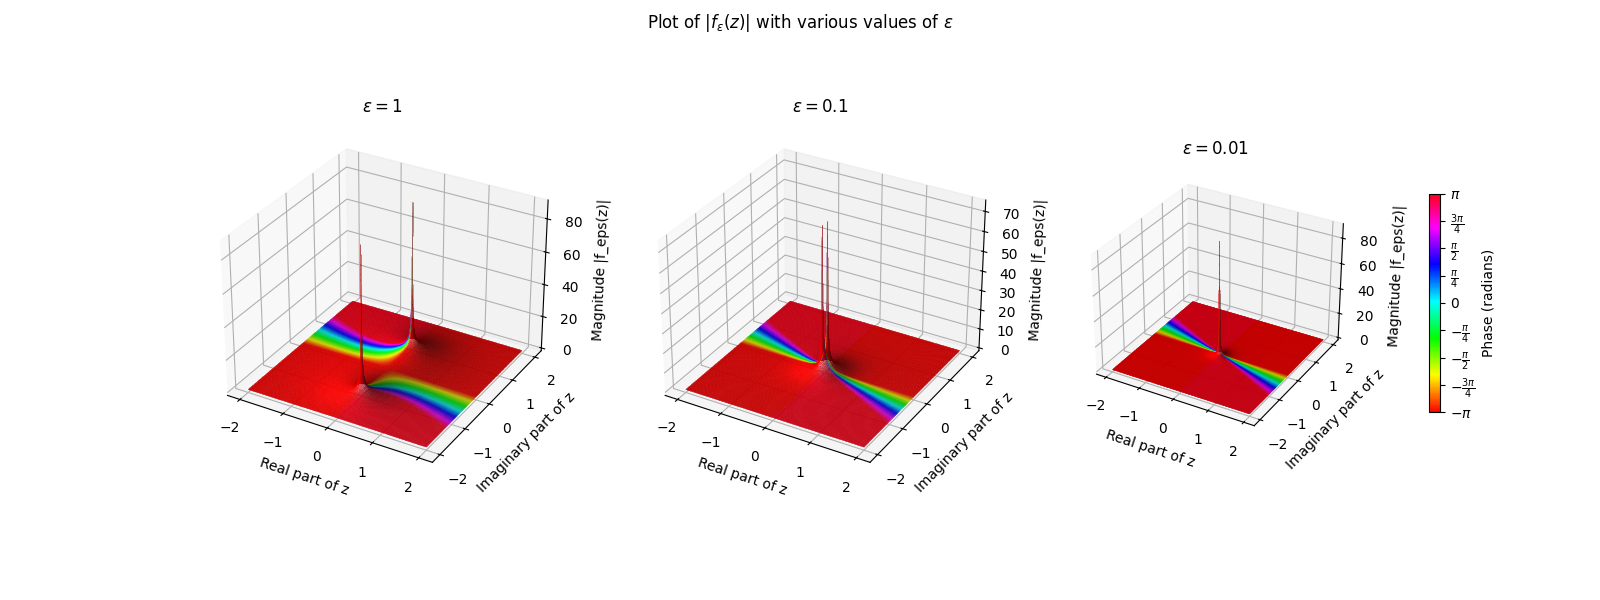
\includegraphics[width=1\textwidth]{f_sub_epsilon_vis.png}
 	\caption{Plot $\left|f_\epsilon(z)\right| = \left| \frac{\epsilon}{\epsilon^2+z^2}\right|$, for various values of $\epsilon$.}\label{fig:f1}
\end{figure}

\noindent
Now to compute the integral we will use the substation $x = \epsilon \tan \theta$ and $\D x = \epsilon \sec^2 \theta \D \theta$
\begin{eqnarray*}
\int_{-\infty}^\infty f_\epsilon(x) \D x = \int_{-\infty}^\infty \frac{\epsilon} {\epsilon^2+x^2} \D x = \int_{-\frac{\pi}{2}}^{\frac{\pi}{2}} \frac{\epsilon^2 \sec^2 \theta} {\epsilon^2 + \epsilon^2 \tan^2\theta}  \D \theta.
\end{eqnarray*}
We get the bounds of the new integral since the following hold $$-\infty = \epsilon \tan \theta \implies \theta = -\frac{\pi}{2} \quad \text{and} \quad \infty = \epsilon \tan \theta \implies \theta = \frac{\pi}{2}.$$
Continuing to solve the new integral
\begin{eqnarray*}
\int_{-\frac{\pi}{2}}^{\frac{\pi}{2}} \frac{\epsilon^2 \sec^2 \theta} {\epsilon^2 + \epsilon^2 \tan^2\theta}  \D \theta &=& \int_{-\frac{\pi}{2}}^{\frac{\pi}{2}} \frac{\epsilon^2 \sec^2 \theta} {\epsilon^2 \left(1 + \tan^2\theta\right)}  \D \theta \\ \\
&=& \int_{-\frac{\pi}{2}}^{\frac{\pi}{2}} \frac{\epsilon^2 }{\epsilon^2 }\frac{\sec^2 \theta} {\sec^2 \theta}  \D \theta \\ \\
&=& \int_{-\frac{\pi}{2}}^{\frac{\pi}{2}} \D \theta \\ \\
&=& \left. \theta \right|_{-\frac{\pi}{2}}^{\frac{\pi}{2}} \\ \\
&=& \frac{\pi}{2} - \left(-\frac{\pi}{2}\right) \\ \\
&=& \pi.
\end{eqnarray*}
\qed \\

\item Visualizing complex functions is not as easy as visualizing
  real-valued functions, since we need 4 dimensions: two for the input,
  two for the output. Different visualizations are commonly used, such
  as showing 3-dimensional plots of the real and imaginary
  parts. Plotting the modulus is informational, but it eliminates a
  lot of information.
  \begin{itemize}
\item To see this, plot the real and imaginary part of the exponential function $\exp (z)=\exp (x+\I y)$, for $x \in[-1,1], y \in[-2 \pi, 2 \pi]$. Now plot the modulus over the same region, and compare.
\item A "new" popular way to do this is to plot the modulus of the
function with the color defined by the phase. The \href{https://dlmf.nist.gov/}{Digital Library of
Mathematical Functions} has lots of examples. Create a plot of the
$|\exp (z)|=|\exp (x+\I y)|$, for $x \in[-1,1]$, $y \in[-2 \pi, 2
\pi]$. colored by the argument. Experimenting with other functions is
highly encouraged! The book visual Complex Functions: An Introduction
with Phase Portraits by Elias Wegert (Birkhäuser, 2012) is a good
companion to our textbook, if you think geometrically.
\end{itemize}
\begin{figure}[h]
	\centering
	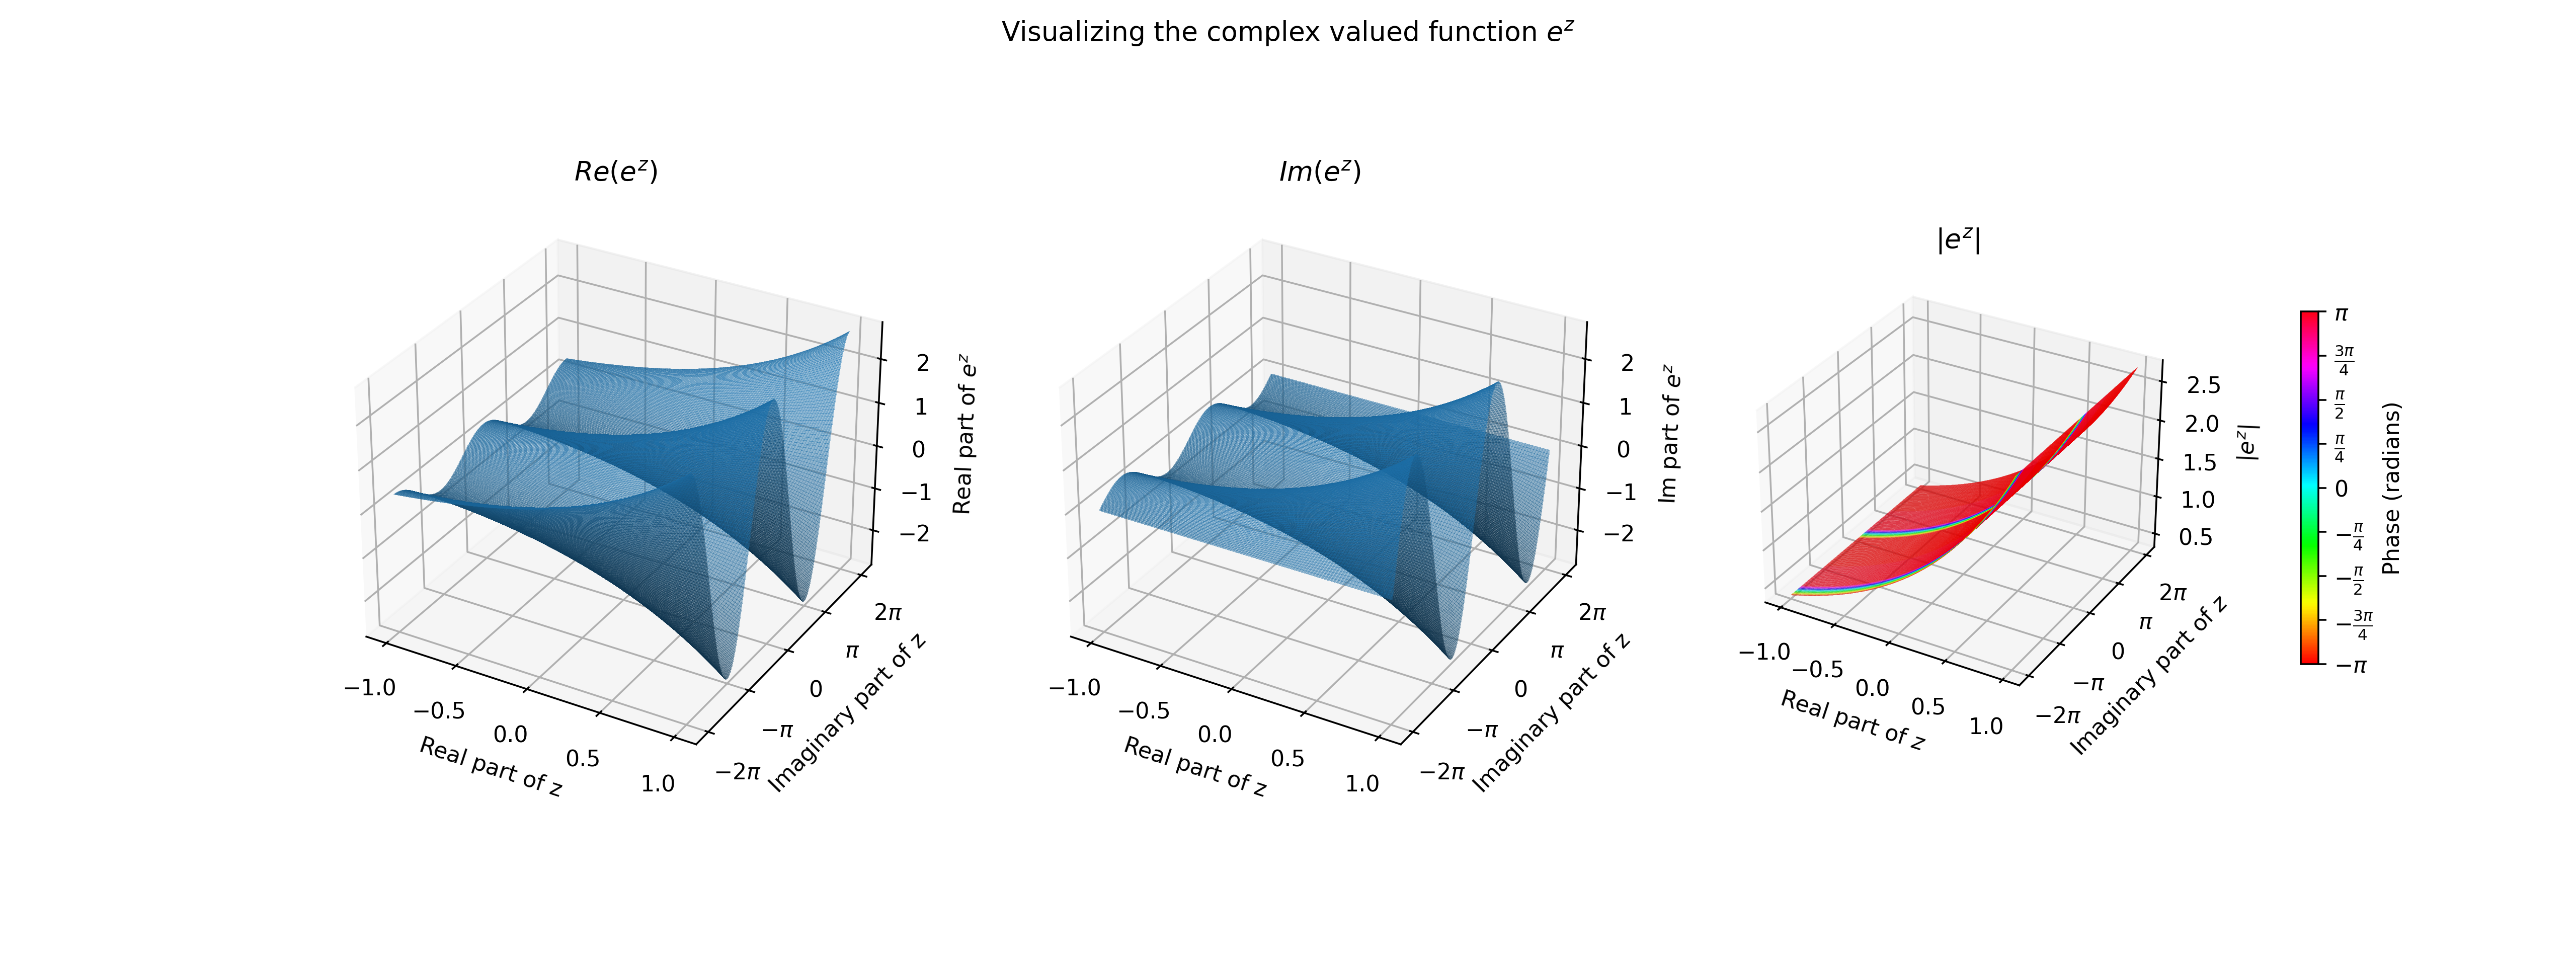
\includegraphics[width=1\textwidth]{exp_z_vis.png}
 	\caption{
		We plot the real and imaginary part of the exponential function $\exp (z)=\exp (x+\I y)$, for $x \in[-1,1], y \in[-2 \pi, 2 \pi]$.
		We also plot the modulus over the same region to compare.
		This all corresponds to problem 6.
	}\label{fig:f2}
\end{figure}
\textit{Solution:} \\
In Figure~\ref{fig:f2} I included all the plots needed for problem 6.
That includes the real and imaginary parts of $e^z$ as well as the modulus of $|e^z|$ with colors corresponding to the phase or $\arg z$. \\
\qed

\item From A\&F: 2.1.1 \\
Which of the following satisfy the Cauchy-Riemann (C-R) equations? If they satisfy the C-R equations, give the analytic function of z. \\
a) $f(x, y) = x - iy + 1$ \\
\textit{Solution:} \\
Identify $u$ and $v$ and their partial derivatives
$$ u(x,y) = x + 1 \implies u_x = 1, \: u_y = 0$$
$$v(x,y) = - y \implies v_x = 0, \: v_y = -1$$
Therefore, $v_x = 0 = - 0 = - u_y$ holds, however $u_x = 1 \neq - 1 = v_y$ does not hold.
In conclusion $f(x, y) = x - iy + 1$ does not satisfy the Cauchy-Riemann (C-R) equations.\\
\qed

\noindent
b) $f(x, y) = y^3 - 3x^2y + i(x^3 - 3xy^2 + 2)$ \\
\textit{Solution:} \\
Identify $u$ and $v$ and their partial derivatives
$$ u(x,y) = y^3 - 3x^2y \implies u_x = -6xy, \: u_y = 3y^2 -3x^2$$
$$v(x,y) = x^3 - 3xy^2 + 2 \implies v_x = 3x^2 - 3y^2, \: v_y = -6xy$$
Therefore, $v_x = 3x^2 - 3y^2 = - (3y^2 -3x^2) = - u_y$ and $u_x = -6xy = -6xy = v_y$ both hold.
In conclusion $f(x, y) = y^3 - 3x^2y + i(x^3 - 3xy^2 + 2)$ satisfies the Cauchy-Riemann (C-R) equations.
To determine the analytic function notice
\begin{eqnarray*}
f(x, y) &=& y^3 - 3x^2y + i(x^3 - 3xy^2 + 2) \\
	 &=& y^3 - 3x^2y + ix^3 - i3xy^2 + i2
\end{eqnarray*}
\begin{eqnarray*}
z^3 &=& (x + iy)^3 \\
      &=& (x + iy)(x + iy)(x + iy) \\
      &=& (x^2 + i2xy - y^2)(x + iy) \\
      &=& x^3 + i3x^2y - 3xy^2 - iy^3 \\
      &=& -i(ix^3 - 3x^2y - i3xy^2 + y^3) \\
      &=& -i(y^3 - 3x^2y + ix^3 - i3xy^2) \\
      &=& -i(f(x,y) - 2i).
\end{eqnarray*}
Continuing
\begin{eqnarray*}
z^3 &=& -i(f(x,y) - 2i) \\
\frac{z^3}{-i} &=& f(x,y) - 2i \\
\frac{z^3}{-i}\frac{i}{i} &=& f(x,y) - 2i \\
iz^3 &=& f(x,y) - 2i \\
iz^3 + 2i &=& f(x,y).
\end{eqnarray*}
Therefore, the analytic function of $z$ is $f(z) = iz^3 + 2i$. \\
\qed

\noindent
c) $f(x, y) = e^y(\cos x + i\sin y)$ \\
\textit{Solution:} \\
Identify $u$ and $v$ and their partial derivatives
$$ f(x, y) = e^y(\cos x + i\sin y) = e^y\cos x + ie^y\sin y $$
$$ u(x,y) = e^y\cos x \implies u_x = -e^y \sin x, \: u_y = e^y\cos x $$
$$ v(x,y) = e^y\sin y \implies v_x = 0, \: v_y = e^y\sin y + e^y \cos y $$
Therefore neither
$$v_x = 0 \neq - e^y\cos x = - u_y$$ nor $$u_x = -e^y \sin x \neq e^y\sin y + e^y \cos y = v_y$$ hold.
In conclusion $f(x, y) = e^y(\cos x + i\sin y)$ does not satisfy the Cauchy-Riemann (C-R) equations. \\
\qed
\item From A\&F: 2.1.7 \\
Consider the complex analytic function, $\Omega(z) = \phi(x, y) + i\psi(x, y)$, in a domain $D$.
Let us transform from $z$ to $w$ using $w = f(z)$, $w = u + iv$ where $f(z)$ is analytic in $D$, with the corresponding domain in the $w$ plane, $D'$.
Establish the following: \\
\textbf{Part 1:}
$$
\frac{\partial\phi}{\partial x} = \frac{\partial u}{\partial x} \frac{\partial\phi}{\partial u} + \frac{\partial v}{\partial x} \frac{\partial\phi}{\partial v}
$$
\textit{Solution:}\\
Notation is very important for this problem. 
Notice the problem sets up that $f(z) = w$ where $w = u + iv$.
We typically say $f(z)$ can be written in a form s.t. $f(z) = u(x,y) + iv(x, y)$ so we really have $f(z) = w = u(x,y) + iv(x,y)$ where $x$ and $y$ are the real and imaginary parts of $z$, respectively.
This gives us \\
$$
\Omega(f(z)) = \Omega(w) = \phi(u(x, y), v(x, y)) + i\psi(u(x, y), v(x, y)).
$$ \\
Therefore we arrive at a function $\phi(u(x, y), v(x, y))$.
Taking the derivative of this with respect to $x$ requires the chain rule.
Applying the chain rule once, we immediately get the following \\
$$\frac{\partial\phi}{\partial x} = \frac{\partial\phi}{\partial u} \frac{\partial u}{\partial x} + \frac{\partial\phi}{\partial v} \frac{\partial v}{\partial x}.$$
\qed \\
\textbf{Part 2:}
\begin{eqnarray*}
\frac{\partial^2\phi}{\partial x^2} &=& \frac{\partial^2 u}{\partial x^2} \frac{\partial\phi}{\partial u}
							- \frac{\partial^2 u}{\partial x \partial y} \frac{\partial\phi}{\partial v}
							+ \left(\frac{\partial v}{\partial x}\right)^2 \frac{\partial^2 \phi}{\partial u^2}
							- 2 \frac{\partial u}{\partial x} \frac{\partial u}{\partial y} \frac{\partial^2 \phi}{\partial u \partial v}
							+ \left(\frac{\partial u}{\partial y}\right)^2 \frac{\partial^2 \phi}{\partial v^2} \\
\end{eqnarray*}
\textit{Solution:} \\
Starting from our previous result
\begin{eqnarray*}
\frac{\partial\phi}{\partial x} &=& \frac{\partial\phi}{\partial u} \frac{\partial u}{\partial x} + \frac{\partial\phi}{\partial v} \frac{\partial v}{\partial x} \\ \\
\frac{\partial}{\partial x} \left(\frac{\partial\phi}{\partial x}\right) &=& \frac{\partial}{\partial x} \left(\frac{\partial\phi}{\partial u} \frac{\partial u}{\partial x} + \frac{\partial\phi}{\partial v} \frac{\partial v}{\partial x}\right) \\ \\
\frac{\partial^2\phi}{\partial x^2} &=& \frac{\partial}{\partial x} \left(\frac{\partial\phi}{\partial u} \frac{\partial u}{\partial x} + \frac{\partial\phi}{\partial v} \frac{\partial v}{\partial x}\right) \\ \\
						&=& \frac{\partial}{\partial x} \left(\frac{\partial\phi}{\partial u} \frac{\partial u}{\partial x}\right)
							+ \frac{\partial}{\partial x}  \left(\frac{\partial\phi}{\partial v} \frac{\partial v}{\partial x}\right) \\ \\
						&=& \left[ 
							\frac{\partial}{\partial x} \left( \frac{\partial\phi}{\partial u} \right) \cdot \frac{\partial u}{\partial x}
							+ \frac{\partial\phi}{\partial u} \cdot \frac{\partial}{\partial x} \left(\frac{\partial u}{\partial x} \right)
						\right]
							+ \left[ 
							\frac{\partial}{\partial x} \left( \frac{\partial\phi}{\partial v} \right) \cdot \frac{\partial v}{\partial x}
							+ \frac{\partial\phi}{\partial v} \cdot \frac{\partial}{\partial x} \left(\frac{\partial v}{\partial x} \right)
						\right] \\ \\
						&=& \left[ 
							\left( \frac{\partial^2 \phi}{\partial u^2} \frac{\partial u}{\partial x} + \frac{\partial^2 \phi}{\partial u \partial v} \frac{\partial v}{\partial x} \right) \frac{\partial u}{\partial x}
							+ \frac{\partial\phi}{\partial u} \frac{\partial^2 u}{\partial x^2}
						\right] 
							+ \left[ 
							\left( \frac{\partial^2 \phi}{\partial v \partial u} \frac{\partial u}{\partial x} + \frac{\partial^2 \phi}{\partial v^2} \frac{\partial v}{\partial x} \right) \frac{\partial v}{\partial x}
							+ \frac{\partial\phi}{\partial v} \frac{\partial^2 v}{\partial x^2}
						\right] \\ \\
						&=& \frac{\partial^2 \phi}{\partial u^2} \left(\frac{\partial u}{\partial x}\right)^2 + \frac{\partial^2 \phi}{\partial u \partial v} \frac{\partial v}{\partial x} \frac{\partial u}{\partial x}
							+ \frac{\partial\phi}{\partial u} \frac{\partial^2 u}{\partial x^2} 
							+ \frac{\partial^2 \phi}{\partial v \partial u} \frac{\partial u}{\partial x}\frac{\partial v}{\partial x} + \frac{\partial^2 \phi}{\partial v^2} \left(\frac{\partial v}{\partial x}\right)^2
							+ \frac{\partial\phi}{\partial v} \frac{\partial^2 v}{\partial x^2} \\ \\
\end{eqnarray*}
Now let's utilize the fact that $f(z)$ is analytic therefore it satisfies the Cauchy-Riemann equations implying
$$\frac{\partial u}{\partial x} = \frac{\partial v}{\partial y} \quad \text{and} \quad \frac{\partial v}{\partial x} = - \frac{\partial u}{\partial y}.$$
Making use of the second equality we proceed in our calculation of $\frac{\partial^2\phi}{\partial x^2}$ by making few substitutions
\begin{eqnarray*}
\frac{\partial^2\phi}{\partial x^2} &=& \frac{\partial^2 \phi}{\partial u^2} \left(\frac{\partial u}{\partial x}\right)^2 + \frac{\partial^2 \phi}{\partial u \partial v} \left(- \frac{\partial u}{\partial y}\right) \frac{\partial u}{\partial x}
							+ \frac{\partial\phi}{\partial u} \frac{\partial^2 u}{\partial x^2} \\
						&& + \frac{\partial^2 \phi}{\partial v \partial u} \frac{\partial u}{\partial x}\left(- \frac{\partial u}{\partial y}\right) + \frac{\partial^2 \phi}{\partial v^2} \left(- \frac{\partial u}{\partial y}\right)^2
							+ \frac{\partial\phi}{\partial v} \frac{\partial^2 v}{\partial x^2} \\ \\
						&=& \frac{\partial^2 \phi}{\partial u^2} \left(\frac{\partial u}{\partial x}\right)^2
							- 2 \frac{\partial u}{\partial x} \frac{\partial u}{\partial y} \frac{\partial^2 \phi}{\partial u \partial v}
							+ \frac{\partial\phi}{\partial u} \frac{\partial^2 u}{\partial x^2}
							+ \frac{\partial^2 \phi}{\partial v^2} \left(\frac{\partial u}{\partial y}\right)^2
							+ \frac{\partial\phi}{\partial v} \frac{\partial^2 v}{\partial x^2} \\ \\
						&=& \frac{\partial\phi}{\partial u} \frac{\partial^2 u}{\partial x^2}
							+ \frac{\partial\phi}{\partial v} \frac{\partial^2 v}{\partial x^2}
							+  \left(\frac{\partial u}{\partial x}\right)^2 \frac{\partial^2 \phi}{\partial u^2}
							- 2 \frac{\partial u}{\partial x} \frac{\partial u}{\partial y} \frac{\partial^2 \phi}{\partial u \partial v}
							+  \left(\frac{\partial u}{\partial y}\right)^2\frac{\partial^2 \phi}{\partial v^2} \\
						&=& \frac{\partial\phi}{\partial u} \frac{\partial^2 u}{\partial x^2}
							+ \frac{\partial\phi}{\partial v}  \frac{\partial}{\partial x} \left(\frac{\partial v}{\partial x}\right)
							+  \left(\frac{\partial u}{\partial x}\right)^2 \frac{\partial^2 \phi}{\partial u^2}
							- 2 \frac{\partial u}{\partial x} \frac{\partial u}{\partial y} \frac{\partial^2 \phi}{\partial u \partial v}
							+  \left(\frac{\partial u}{\partial y}\right)^2\frac{\partial^2 \phi}{\partial v^2} \\
						&=& \frac{\partial\phi}{\partial u} \frac{\partial^2 u}{\partial x^2}
							+ \frac{\partial\phi}{\partial v}  \frac{\partial}{\partial x} \left(- \frac{\partial u}{\partial y}\right)
							+  \left(\frac{\partial u}{\partial x}\right)^2 \frac{\partial^2 \phi}{\partial u^2}
							- 2 \frac{\partial u}{\partial x} \frac{\partial u}{\partial y} \frac{\partial^2 \phi}{\partial u \partial v}
							+  \left(\frac{\partial u}{\partial y}\right)^2\frac{\partial^2 \phi}{\partial v^2} \\
						&=& \frac{\partial\phi}{\partial u} \frac{\partial^2 u}{\partial x^2}
							- \frac{\partial\phi}{\partial v} \frac{\partial^2 u}{\partial x \partial y}
							+  \left(\frac{\partial u}{\partial x}\right)^2 \frac{\partial^2 \phi}{\partial u^2}
							- 2 \frac{\partial u}{\partial x} \frac{\partial u}{\partial y} \frac{\partial^2 \phi}{\partial u \partial v}
							+  \left(\frac{\partial u}{\partial y}\right)^2\frac{\partial^2 \phi}{\partial v^2}.
\end{eqnarray*}
\qed \\
\noindent
\textbf{Part 3:} 
Also find the corresponding formulae for $\frac{\partial \phi}{\partial y}$ and $\frac{\partial^2 \phi }{\partial y^2}$. \\
\textit{Solution:} \\
Recall that we are looking at $\phi(u(x, y), v(x, y))$\\
Taking the derivative of this with respect to $y$ requires the chain rule.
Applying the chain rule once, we immediately get the following \\
$$\frac{\partial\phi}{\partial y} = \frac{\partial\phi}{\partial u} \frac{\partial u}{\partial y} + \frac{\partial\phi}{\partial v} \frac{\partial v}{\partial y}.$$
And now continuing on with the second derivative we get:
\begin{eqnarray*}
\frac{\partial\phi}{\partial y} &=& \frac{\partial\phi}{\partial u} \frac{\partial u}{\partial y} + \frac{\partial\phi}{\partial v} \frac{\partial v}{\partial y} \\ \\
\frac{\partial}{\partial y} \left(\frac{\partial\phi}{\partial y}\right) &=& \frac{\partial}{\partial y} \left(\frac{\partial\phi}{\partial u} \frac{\partial u}{\partial y} + \frac{\partial\phi}{\partial v} \frac{\partial v}{\partial y}\right) \\ \\
\frac{\partial^2\phi}{\partial y^2} &=& \frac{\partial}{\partial y} \left(\frac{\partial\phi}{\partial u} \frac{\partial u}{\partial y} + \frac{\partial\phi}{\partial v} \frac{\partial v}{\partial y}\right) \\ \\
						&=& \frac{\partial}{\partial y} \left(\frac{\partial\phi}{\partial u} \frac{\partial u}{\partial y}\right)
							+ \frac{\partial}{\partial y}  \left(\frac{\partial\phi}{\partial v} \frac{\partial v}{\partial y}\right) \\ \\
						&=& \left[ 
							\frac{\partial}{\partial y} \left( \frac{\partial\phi}{\partial u} \right) \cdot \frac{\partial u}{\partial y}
							+ \frac{\partial\phi}{\partial u} \cdot \frac{\partial}{\partial y} \left(\frac{\partial u}{\partial y} \right)
						\right] 
							+ \left[ 
							\frac{\partial}{\partial y} \left( \frac{\partial\phi}{\partial v} \right) \cdot \frac{\partial v}{\partial y}
							+ \frac{\partial\phi}{\partial v} \cdot \frac{\partial}{\partial y} \left(\frac{\partial v}{\partial y} \right)
						\right] \\ \\
						&=& \left[ 
							\left( \frac{\partial^2 \phi}{\partial u^2} \frac{\partial u}{\partial y} + \frac{\partial^2 \phi}{\partial u \partial v} \frac{\partial v}{\partial y} \right) \frac{\partial u}{\partial y}
							+ \frac{\partial\phi}{\partial u} \frac{\partial^2 u}{\partial y^2}
						\right] 
							+ \left[ 
							\left( \frac{\partial^2 \phi}{\partial v \partial u} \frac{\partial u}{\partial y} + \frac{\partial^2 \phi}{\partial v^2} \frac{\partial v}{\partial y} \right) \frac{\partial v}{\partial y}
							+ \frac{\partial\phi}{\partial v} \frac{\partial^2 v}{\partial y^2}
						\right] \\ \\
						&=& \frac{\partial^2 \phi}{\partial u^2} \left(\frac{\partial u}{\partial y}\right)^2 + \frac{\partial^2 \phi}{\partial u \partial v} \frac{\partial v}{\partial y} \frac{\partial u}{\partial y}
							+ \frac{\partial\phi}{\partial u} \frac{\partial^2 u}{\partial y^2} 
							+ \frac{\partial^2 \phi}{\partial v \partial u} \frac{\partial u}{\partial y}\frac{\partial v}{\partial y} + \frac{\partial^2 \phi}{\partial v^2} \left(\frac{\partial v}{\partial y}\right)^2
							+ \frac{\partial\phi}{\partial v} \frac{\partial^2 v}{\partial y^2} \\ \\
\end{eqnarray*}
We need to decide where our substitutions are going to take place
\begin{eqnarray*}
\frac{\partial^2\phi}{\partial y^2} &=& \frac{\partial^2 \phi}{\partial u^2} \left(\frac{\partial u}{\partial y}\right)^2 + \frac{\partial^2 \phi}{\partial u \partial v} \frac{\partial v}{\partial y} \left(- \frac{\partial v}{\partial x}\right)
							+ \frac{\partial\phi}{\partial u} \frac{\partial}{\partial y} \left(- \frac{\partial v}{\partial x} \right)\\ \\
						&& + \frac{\partial^2 \phi}{\partial v \partial u} \left(- \frac{\partial v}{\partial x}\right)\frac{\partial v}{\partial y} + \frac{\partial^2 \phi}{\partial v^2} \left(\frac{\partial v}{\partial y}\right)^2
							+ \frac{\partial\phi}{\partial v} \frac{\partial^2 v}{\partial y^2} \\ \\
						&=& \frac{\partial^2 \phi}{\partial u^2} \left(\frac{\partial u}{\partial y}\right)^2
							-2 \frac{\partial^2 \phi}{\partial u \partial v} \frac{\partial v}{\partial y} \frac{\partial v}{\partial x}
							- \frac{\partial\phi}{\partial u} \frac{\partial^2 v}{\partial x \partial y}
							+ \frac{\partial^2 \phi}{\partial v^2} \left(\frac{\partial v}{\partial y}\right)^2
							+ \frac{\partial\phi}{\partial v} \frac{\partial^2 v}{\partial y^2} \\ \\
						&=& \frac{\partial\phi}{\partial v} \frac{\partial^2 v}{\partial y^2} 
							- \frac{\partial\phi}{\partial u} \frac{\partial^2 v}{\partial x \partial y}
							+ \left(\frac{\partial u}{\partial y}\right)^2 \frac{\partial^2 \phi}{\partial u^2}
							-2 \frac{\partial^2 \phi}{\partial u \partial v} \frac{\partial v}{\partial y} \frac{\partial v}{\partial x}
							+ \left(\frac{\partial v}{\partial y}\right)^2 \frac{\partial^2 \phi}{\partial v^2}. \\ \\
\end{eqnarray*}
Therefore we have derived the similar formula for $\frac{\partial^2 \phi }{\partial y^2}$ as we had for $\frac{\partial^2 \phi }{\partial x^2}$.
\qed \\

\noindent
\textbf{Part 3:}  Recall that $f'(z) = \frac{\partial u }{\partial x} + i\frac{\partial u}{\partial y}$, and $u(x, y)$ satisfies Laplace's equation the domain D.
Show that
$$
\nabla_{x, y}^2 \phi = 
\frac{\partial^2\phi}{\partial x^2} + \frac{\partial^2 \phi }{\partial y^2} = 
\left(u_x^2 + y_y^2\right) \left(\frac{\partial^2\phi}{\partial u^2} + \frac{\partial^2 \phi }{\partial v^2}\right) =
\left| f'(z)\right|^2 \nabla_{u, v}^2 \phi
$$
\textit{Solution:}
The first equality comes by definition of $\nabla_{x, y}^2 \phi$.
Similarly the third equality comes from the definition of $f'(z)$, the modulus and $\nabla_{u, v}^2 \phi$.
So what we really need to show is that
$$
\frac{\partial^2\phi}{\partial x^2} + \frac{\partial^2 \phi }{\partial y^2} = 
\left(u_x^2 + u_y^2\right) \left(\frac{\partial^2\phi}{\partial u^2} + \frac{\partial^2 \phi }{\partial v^2}\right).
$$
Lets get to it
\begin{eqnarray*}
\frac{\partial^2\phi}{\partial x^2} + \frac{\partial^2 \phi }{\partial y^2} &=& \left[\frac{\partial\phi}{\partial u} \frac{\partial^2 u}{\partial x^2}
													- \frac{\partial\phi}{\partial v} \frac{\partial^2 u}{\partial x \partial y}
													+  \left(\frac{\partial u}{\partial x}\right)^2 \frac{\partial^2 \phi}{\partial u^2}
													-2 \frac{\partial u}{\partial x} \frac{\partial u}{\partial y} \frac{\partial^2 \phi}{\partial u \partial v}
													+  \left(\frac{\partial u}{\partial y}\right)^2\frac{\partial^2 \phi}{\partial v^2} \right] \\ \\
												  && + \left[\frac{\partial\phi}{\partial v} \frac{\partial^2 v}{\partial y^2} 
													- \frac{\partial\phi}{\partial u} \frac{\partial^2 v}{\partial x \partial y}
													+ \left(\frac{\partial u}{\partial y}\right)^2 \frac{\partial^2 \phi}{\partial u^2}
													-2 \frac{\partial^2 \phi}{\partial u \partial v} \frac{\partial v}{\partial y} \frac{\partial v}{\partial x}
													+ \left(\frac{\partial v}{\partial y}\right)^2 \frac{\partial^2 \phi}{\partial v^2} \right]\\ \\
												   &=& \frac{\partial\phi}{\partial u} \frac{\partial^2 u}{\partial x^2}
													+ \frac{\partial\phi}{\partial v} \frac{\partial^2 v}{\partial y^2} 
													- \frac{\partial\phi}{\partial v} \frac{\partial^2 u}{\partial x \partial y}
													- \frac{\partial\phi}{\partial u} \frac{\partial^2 v}{\partial x \partial y}
													-2 \frac{\partial u}{\partial x} \frac{\partial u}{\partial y} \frac{\partial^2 \phi}{\partial u \partial v}
													-2 \frac{\partial^2 \phi}{\partial u \partial v} \frac{\partial v}{\partial y} \frac{\partial v}{\partial x} \\ \\
												   && +  \left(\frac{\partial u}{\partial x}\right)^2 \frac{\partial^2 \phi}{\partial u^2}
													+ \left(\frac{\partial u}{\partial y}\right)^2 \frac{\partial^2 \phi}{\partial u^2}
													+ \left(\frac{\partial v}{\partial y}\right)^2 \frac{\partial^2 \phi}{\partial v^2} 
													+  \left(\frac{\partial u}{\partial y}\right)^2\frac{\partial^2 \phi}{\partial v^2} \\ \\
												   &=& \frac{\partial\phi}{\partial u} \frac{\partial^2 u}{\partial x^2}
													+ \frac{\partial\phi}{\partial v} \frac{\partial^2 v}{\partial y^2} 
													- \frac{\partial\phi}{\partial v} \frac{\partial^2 u}{\partial x \partial y}
													- \frac{\partial\phi}{\partial u} \frac{\partial^2 v}{\partial x \partial y}
													-2 \frac{\partial u}{\partial x} \frac{\partial u}{\partial y} \frac{\partial^2 \phi}{\partial u \partial v}
													-2 \frac{\partial^2 \phi}{\partial u \partial v} \frac{\partial v}{\partial y} \frac{\partial v}{\partial x} \\ \\
												    && +  \left(\frac{\partial u}{\partial x}\right)^2 \frac{\partial^2 \phi}{\partial u^2}
												        	 + \left(\frac{\partial u}{\partial y}\right)^2 \frac{\partial^2 \phi}{\partial u^2}
													 + \left(\frac{\partial v}{\partial y}\right)^2 \frac{\partial^2 \phi}{\partial v^2} 
													 + \left(\frac{\partial u}{\partial y}\right)^2\frac{\partial^2 \phi}{\partial v^2} \\ \\
												&=& \frac{\partial\phi}{\partial u} \frac{\partial^2 u}{\partial x^2}
													+ \frac{\partial\phi}{\partial v} \frac{\partial^2 v}{\partial y^2} 
													- \frac{\partial\phi}{\partial v} \frac{\partial^2 u}{\partial x \partial y}
													- \frac{\partial\phi}{\partial u} \frac{\partial^2 v}{\partial x \partial y}
													-2 \frac{\partial u}{\partial x} \frac{\partial u}{\partial y} \frac{\partial^2 \phi}{\partial u \partial v}
													+2 \frac{\partial^2 \phi}{\partial u \partial v} \frac{\partial u}{\partial x} \frac{\partial u}{\partial y} \\ \\
												    && +  \left(\frac{\partial u}{\partial x}\right)^2 \frac{\partial^2 \phi}{\partial u^2}
												        	 + \left(\frac{\partial u}{\partial y}\right)^2 \frac{\partial^2 \phi}{\partial u^2}
													 + \left(\frac{\partial v}{\partial y}\right)^2 \frac{\partial^2 \phi}{\partial v^2} 
													 + \left(\frac{\partial u}{\partial y}\right)^2\frac{\partial^2 \phi}{\partial v^2} \\ \\
												&=& \frac{\partial\phi}{\partial u} \frac{\partial^2 u}{\partial x^2}
													- \frac{\partial\phi}{\partial u} \frac{\partial^2 v}{\partial x \partial y} 
													+ \frac{\partial\phi}{\partial v} \frac{\partial^2 v}{\partial y^2} 
													- \frac{\partial\phi}{\partial v} \frac{\partial^2 u}{\partial x \partial y}\\ \\
												    && +  \left(\frac{\partial u}{\partial x}\right)^2 \frac{\partial^2 \phi}{\partial u^2}
												        	 + \left(\frac{\partial u}{\partial y}\right)^2 \frac{\partial^2 \phi}{\partial u^2}
													 + \left(\frac{\partial v}{\partial y}\right)^2 \frac{\partial^2 \phi}{\partial v^2} 
													 + \left(\frac{\partial u}{\partial y}\right)^2\frac{\partial^2 \phi}{\partial v^2} \\ \\
\end{eqnarray*}
Now using substitutions from the C-R equations again
\begin{eqnarray*}
\frac{\partial^2\phi}{\partial x^2} + \frac{\partial^2 \phi }{\partial y^2} &=& \frac{\partial\phi}{\partial u} \left(\frac{\partial^2 u}{\partial x^2} - \frac{\partial^2 v}{\partial x \partial y} \right)
													+ \frac{\partial\phi}{\partial v} \left(\frac{\partial^2 v}{\partial y^2} - \frac{\partial^2 u}{\partial x \partial y} \right)\\ \\
												    && +  \left(\frac{\partial u}{\partial x}\right)^2 \frac{\partial^2 \phi}{\partial u^2}
												        	 + \left(\frac{\partial u}{\partial y}\right)^2 \frac{\partial^2 \phi}{\partial u^2}
													 + \left(\frac{\partial v}{\partial y}\right)^2 \frac{\partial^2 \phi}{\partial v^2} 
													 + \left(\frac{\partial u}{\partial y}\right)^2\frac{\partial^2 \phi}{\partial v^2} \\ \\
												&=& \frac{\partial\phi}{\partial u} \left(\frac{\partial^2 u}{\partial x^2} - \frac{\partial}{\partial x} \left(\frac{\partial v}{\partial y} \right)\right)
													+ \frac{\partial\phi}{\partial v} \left(\frac{\partial^2 v}{\partial y^2} - \frac{\partial}{\partial y} \left(\frac{\partial u}{\partial x} \right) \right) \\ \\
												    && +  \left(\frac{\partial u}{\partial x}\right)^2 \frac{\partial^2 \phi}{\partial u^2}
												        	 + \left(\frac{\partial u}{\partial y}\right)^2 \frac{\partial^2 \phi}{\partial u^2}
													 + \left(\frac{\partial v}{\partial y}\right)^2 \frac{\partial^2 \phi}{\partial v^2} 
													 + \left(\frac{\partial u}{\partial y}\right)^2\frac{\partial^2 \phi}{\partial v^2} \\ \\
												&=& \frac{\partial\phi}{\partial u} \left(\frac{\partial^2 u}{\partial x^2} - \frac{\partial}{\partial x} \left(\frac{\partial u}{\partial x} \right)\right)
													+ \frac{\partial\phi}{\partial v} \left(\frac{\partial^2 v}{\partial y^2} - \frac{\partial}{\partial y} \left(\frac{\partial v}{\partial y} \right) \right) \\ \\
												    && +  \left(\frac{\partial u}{\partial x}\right)^2 \frac{\partial^2 \phi}{\partial u^2}
												        	 + \left(\frac{\partial u}{\partial y}\right)^2 \frac{\partial^2 \phi}{\partial u^2}
													 + \left(\frac{\partial v}{\partial y}\right)^2 \frac{\partial^2 \phi}{\partial v^2} 
													 + \left(\frac{\partial u}{\partial y}\right)^2\frac{\partial^2 \phi}{\partial v^2} \\ \\
												&=& \frac{\partial\phi}{\partial u} \left(\frac{\partial^2 u}{\partial x^2} - \frac{\partial^2 u}{\partial x^2} \right)
													+ \frac{\partial\phi}{\partial v} \left(\frac{\partial^2 v}{\partial y^2} - \frac{\partial^2 v}{\partial y^2} \right) \\ \\
												    && +  \left(\frac{\partial u}{\partial x}\right)^2 \frac{\partial^2 \phi}{\partial u^2}
												        	 + \left(\frac{\partial u}{\partial y}\right)^2 \frac{\partial^2 \phi}{\partial u^2}
													 + \left(\frac{\partial v}{\partial y}\right)^2 \frac{\partial^2 \phi}{\partial v^2} 
													 + \left(\frac{\partial u}{\partial y}\right)^2\frac{\partial^2 \phi}{\partial v^2} \\ \\
												&=& \left(\frac{\partial u}{\partial x}\right)^2 \frac{\partial^2 \phi}{\partial u^2}
												        	 + \left(\frac{\partial u}{\partial y}\right)^2 \frac{\partial^2 \phi}{\partial u^2}
													 + \left(\frac{\partial v}{\partial y}\right)^2 \frac{\partial^2 \phi}{\partial v^2} 
													 + \left(\frac{\partial u}{\partial y}\right)^2\frac{\partial^2 \phi}{\partial v^2} \\ \\
												&=& \left(\frac{\partial u}{\partial x}\right)^2 \frac{\partial^2 \phi}{\partial u^2}
												        	 + \left(\frac{\partial u}{\partial y}\right)^2 \frac{\partial^2 \phi}{\partial u^2}
													 + \left(\frac{\partial u}{\partial x}\right)^2 \frac{\partial^2 \phi}{\partial v^2} 
													 + \left(\frac{\partial u}{\partial y}\right)^2\frac{\partial^2 \phi}{\partial v^2} \\ \\
												&=& \left(\frac{\partial u}{\partial x}\right)^2 \frac{\partial^2 \phi}{\partial u^2}
													+ \left(\frac{\partial u}{\partial x}\right)^2 \frac{\partial^2 \phi}{\partial v^2}
												        	 + \left(\frac{\partial u}{\partial y}\right)^2 \frac{\partial^2 \phi}{\partial u^2}												  
													 + \left(\frac{\partial u}{\partial y}\right)^2\frac{\partial^2 \phi}{\partial v^2} \\ \\
												&=& u_x^2\frac{\partial^2\phi}{\partial u^2}
													+ u_x^2\frac{\partial^2 \phi }{\partial v^2}
													+ u_y^2\frac{\partial^2\phi}{\partial u^2}
													+ u_y^2\frac{\partial^2 \phi }{\partial v^2} \\ \\
												&=& \left(u_x^2 + u_y^2\right) \left(\frac{\partial^2\phi}{\partial u^2} + \frac{\partial^2 \phi }{\partial v^2}\right)
\end{eqnarray*}
\qed \\
\noindent
Consequently, we find that if $\phi$ satisfies Laplace's equation $\nabla_{x, y}^2 \phi = 0$ in the domain $D$,
then so long as $f'(z) \neq 0$ in $D$ it also satisfies Laplace's equation $\nabla_{u, v}^2 \phi = 0$ in domain $D'$. \\
\item Show that the derivative of $f(z)=|z|^2$ is defined at $z=0$, but nowhere else.\\
\textit{Solution:} \\
Once again we are going to use the C-R equations and the fact that satisfying them is a necessary condition for differentiability.
\begin{eqnarray*}
f(z) &=&|z|^2 \\
      &=&\sqrt{x^2 + y^2}^2 \\
      &=& x^2 + y^2 \\
      &=& x^2 + y^2 + i \cdot 0
\end{eqnarray*}
Therefore $u(x, y) = x^2 + y^2$ and $v(x, y) = 0$. Now let's calculate the necessary partials
$$u_x = 2x$$ $$v_y = 0$$ $$v_x = 0$$ $$u_y = 2y.$$
Now we need the following to hold for $f(z)$ to be differentiable
\begin{eqnarray*}
u_x &=& v_y \\
2x &=& 0
\end{eqnarray*}
\text{and}
\begin{eqnarray*}
v_x &=& - u_y \\
0 &=& - 2y.
\end{eqnarray*}
Both of these only hold if $x=0$ and $y=0$ or in other words if $z=0$.
Which means the C-R equations only hold at $z=0$ and the derivative of $f(z) = |z|^2$ is defined at $z=0$ but nowhere else. \\
\qed

\item Derive the polar-coordinates form of the Cauchy-Riemann equations
$$
u_r=\frac{1}{r} v_\theta, \quad v_r=-\frac{1}{r} u_\theta.
$$
where $x=r \cos \theta$ and $y=r \sin \theta$ \\
\textit{Solution:} \\
We know we can represent $f(z) = u(x, y) + i v(x, y)$.
Let's make a substitution to polar coordinates
\begin{eqnarray*}
f(z) &=& u(x, y) + i v(x, y) \\
      &=& u(r \cos \theta, r \sin \theta) + i v(r \cos \theta, r \sin \theta) \\
      &=& U(r, \theta) + iV(r, \theta)
\end{eqnarray*}
We need to calculate the derivatives using the chain rule
$$U_r = u_xx_r + u_yy_r$$
$$U_\theta = u_xx_\theta + u_yy_\theta$$
$$V_r = v_xx_r + v_yy_r$$
$$V_\theta = v_xx_\theta + v_yy_\theta.$$

Now we compute the necessary partials and plug them back in
\begin{eqnarray*}
x_r &=& \cos \theta \\
x_\theta &=& - r \sin \theta \\
y_r &=& \sin \theta \\
y_\theta &=& r \cos \theta
\end{eqnarray*}
$$\downarrow$$
\begin{eqnarray*}
U_r &=& u_x \cos \theta + u_y \sin \theta \\
U_\theta &=& - u_x r \sin \theta + u_y r \cos \theta \\
V_r &=& v_x \cos \theta  + v_y  \sin \theta \\
V_\theta &=& - v_x r \sin \theta + v_y r \cos \theta.
\end{eqnarray*}
Now try to make them look like each other with the C-R equations
\begin{eqnarray*}
U_r &=& u_x \cos \theta + u_y \sin \theta \\
       &=& v_y \cos \theta + u_y \sin \theta
\end{eqnarray*}
then
\begin{eqnarray*}
V_\theta &=& - v_x r \sin \theta + v_y r \cos \theta \\
	      &=&  u_y r \sin \theta + v_y r \cos \theta \\
	      &=&  r (u_y \sin \theta + v_y \cos \theta ) \\
	      &=&  r (v_y \cos \theta + u_y \sin \theta) \\
	      &=&  r U_r
\end{eqnarray*}
Therefore $U_r = \frac{1}{r}V_\theta$.
\begin{eqnarray*}
V_r &=& v_x \cos \theta  + v_y  \sin \theta \\
       &=& -u_y \cos \theta  + v_y  \sin \theta
\end{eqnarray*}
then
\begin{eqnarray*}
U_\theta &=& - u_x r \sin \theta + u_y r \cos \theta \\
	      &=& - v_y r \sin \theta + u_y r \cos \theta \\
	      &=& - r (v_y \sin \theta - u_y \cos \theta) \\
	      &=& - r (- u_y \cos \theta + v_y \sin \theta) \\
	      &=& - r V_r
\end{eqnarray*}
Therefore $V_r = - \frac{1}{r}U_\theta$.
And with this we have derived the polar-coordinates form of the Cauchy-Riemann equations. \\
\qed
\end{enumerate}

\end{document}

%%% Local Variables:
%%% mode: latex
%%% TeX-master: t
%%% End:
